\documentclass[12pt]{article}
\usepackage[a4paper, total={6in, 10in}]{geometry}

\usepackage{graphicx}
\usepackage{abstract}
\usepackage{hyperref}
\usepackage{listings}
\usepackage{indentfirst}
\usepackage{amssymb}
\usepackage{titling}
\usepackage{mwe}
\usepackage{fancyhdr}
\usepackage{setspace}

\graphicspath{ {./images/} }
\onehalfspacing

\setlength{\parskip}{3mm}   % Add space between paragraphs.
\setlength{\parindent}{0.5in}
\setlength{\droptitle}{-35pt}

\fancypagestyle{plain}{
    \vspace{3ex}
    \fancyhead[L]{November 14th, 2020}
    \renewcommand{\headrulewidth}{0.5pt}
}

\pretitle{\begin{center} \LARGE \textbf}
\posttitle{\end{center} \vspace{-3ex}}
\preauthor{\begin{center} \large}
\postauthor{\end{center} \vspace{-3ex}}
\predate{\begin{center} \small \emph}
\postdate{\end{center} \vspace{-3ex}}

\title{Chapter 5 Summary \& Review Questions}
\author{Chris Nutter\thanks{Dedicated to @QuesoGrande a.k.a. Jared D.}}
\date{CPSC 315}

% --> Here we go, satellite radio, y'all get hit with a...

\begin{document}
\maketitle

%\begin{center} \vspace{-4ex}|\vspace{-3ex} \end{center}
\normalsize

\tableofcontents    
\vspace{4ex}

\begin{center} Content begins on next page. \end{center}

\newpage
% --> First Chapter

\section{Chapter 5 Summary}
    \indent Privacy is one of the essential human rights and it's something that makes each human feel safe and secure. Each day we progress, our society and government want to invade our privacy more and more in order to make money to people who want the information. Daily people are stripped of their social security, medical information, and phone numbers and sold to corrupt government agents or worse, China.\\
    \indent Modern technology makes it very easy for people to be susceptible to bad privacy standards. Facebook is a prime example of a company who makes a living off of its users giving as much information as possible. It's a scary fact that everyday people are losing social security numbers just because their credit card got "hacked" and the person didn't know better so they give up vital information. We live in a society nowadays where it is so easy to lose a huge chunk of your life.\\
    \indent Many organizations collect information on individuals and plan on selling to third-parties for profit. Any program or social media that they market as "free" will often use each individual as the product and sell the information. Facebook is insanely bad when it comes to their privacy aspects and have been shown to sell information to other people.\\
    \indent This last paragraph will summarize what to do to not get your information sold. Do NOT use social media. Every social media uses your information as a source of payment for the company. Do. Not. Use. Social. Media. Also do not give up your information to anyone. Use safe services to pay people (i.e. Paypal). Lastly, do not go online. That's obviously impossible so here are some nice things that can help you feel safer.
    \begin{enumerate}
       \item Get an Android phone and install a custom ROM with microG. It's a variant of Google Play Services that doesn't use Google and doesn't send traffic. You can block location, market, everything Google related. Very awesome. (Also it's really good on battery).
       \item Use an iPod for music. No Wifi/Ethernet means it cannot get hacked.
       \item USE A VPN. USE A VPN. USE A VPN!!! I recommend Private Internet Access or Mullvad.
       \item Use LastPass to randomly generate passwords.
       \item Do not give up any personal information to anyone. At all. Ever. 
    \end{enumerate}
\newpage
\onehalfspacing

\section{Review Questions}
    \begin{enumerate}
        \item Being alone is the concept of no interaction with the people around you. Privacy is still being able to be around other people however they don't know things you do not want them to know. I prefer privacy but being alone is nice sometimes too.
        \item Excess privacy can lead to bad people running bad practices underneath the knowledge of the government (sex trafficking, looting, etc) while not enough privacy can lead to the knowledge of everyone around us and lead to a very insecure and pressuring society.
        \item Privacy is a prudential right as the philosophy stands that each human has an inherent right to life, liberty, and the pursuit of happiness. Liberty = privacy.
        \item Privacy is a positive right meaning that it's a good thing to have. I firmly believe that privacy should be expressed making it a positive right.
        \item Some information should be made public limited to criminal records so we understand our community and can act accordingly.
        \item One example of where a person has to disclose personal information would be applying for a credit card because your social security is linked to your own credit and using another SS is considered fraud.
        \item Retailers use loyalty cards to improve sales because the cards are to be paid to the companies and loyalty cards on their end add to a credit service.
        \item Personally I see NO benefit of public medical records because that's something I believe no one should disclose unless appropriate. The risks are far and wide. Disclosing medical records could lead to "leaking" of them to companies and targeted ads towards the person with specific diseases. If I get ads based around my medical records, I won't be happy.
        \item Cookies from a web site can be stored and saved on the websites side and could potentially be sold to other companies.
        \item Data mining is the concept of a company taking information from a source while collaborative filtering is the effort of a group getting disclosed information and grabbing the information it needs.
        \item Opt-in policy is where the person MUST say yes or no to a policy at hand while opt-out policy they are AUTOMATICALLY said yes and have to remove themselves.
        \item Be safe on the internet is the real lesson. If you're information is online it's there forever. Be careful. Don't get worried however if you find your email somewhere. If it were really bad, you'd know.
    \end{enumerate}

\end{document} 

% Possibly Important LaTeX Functions %
% ================================== %

%   \begin{figure}[hbtp]
%       \centering
%       \fbox{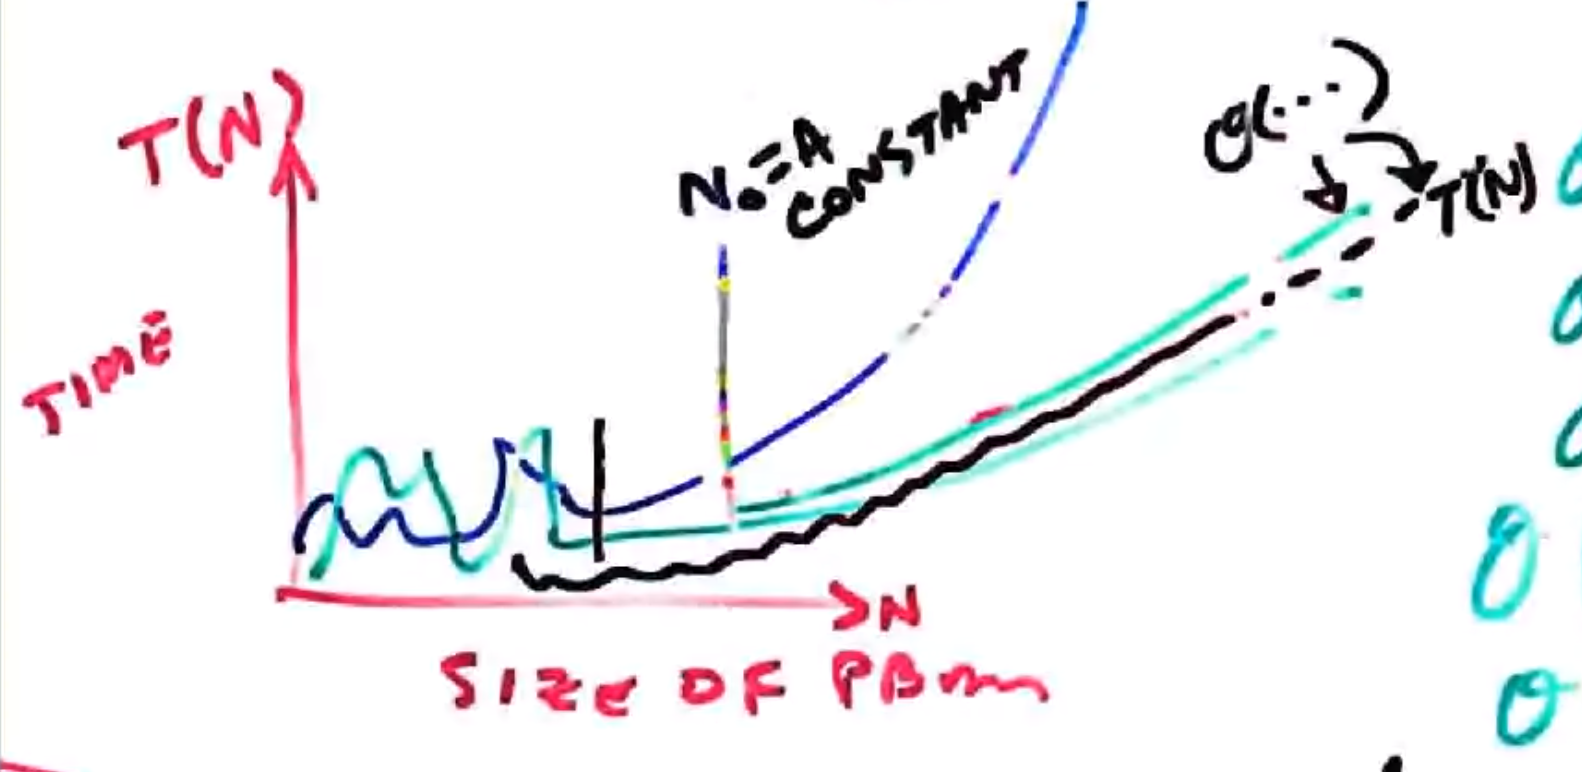
\includegraphics[width=13.8cm]{big_o.png}}
%       \caption{Big(O) Notation}
%   \end{figure}

%   \begin{lstlisting}[language=Python] 
%        print('hello world') 
%   \end{lstlisting}  

